%xelatex -shell-escape -output-directory=bin ergasia.tex
\documentclass{assignment}

\usepackage{enumerate} % Για την χρησιμοποίηση roman enumerate
\usepackage{paralist} % για το περιβάλλον inparaenum που είναι οι λίστες μέσα στο κείμενο.

\title{Ειδικά Θέματα Αντικειμενοστραφούς Προγραμματισμού \\ Θέμα Εξαμήνου}
\date{Αθήνα, 2015}

\author{Αναγνωστόπουλος Βασίλης - Θάνος (ΜΠΠΛ 13002)}

\begin{document}

\maketitle
% Να σκεφτώ τί αλλαγές θέλω να κάνω με τις αριθμήσεις και άμα θέλω να κάνω.
% Να σκεφτώ να τις ενσωματώσω και στο assignment.cls

\setcounter{page}{1} 
\pagenumbering{roman}

\pagestyle{plain}
\tableofcontents
%\listoftables
%\listoffigures
%\renewcommand\listoflistingscaption{Κατάλογος πηγαίου κώδικα}
%\listoflistings
\newpage

%\pagestyle{headings}
%\pagestyle{fancy}
\setcounter{page}{1} 
\pagenumbering{arabic}

\section{Εισαγωγή}

Στην παρούσα εργασία κατασκευάστηκε μία \en{mobile} εφαρμογή με τίτλο "\en{Uni\-pi Alert}". Η συγκεκριμένη εφαρμογή ενημερώνει μέσω γραπτού μηνύματος για την θέση του χρήστη και ότι βρίσκεται σε κάποια κατάσταση εκτάκτου ανάγκης.

\section{Κεντρική οθόνη}

Στο σχήμα \ref{fig:initial_screen} φαίνεται η αρχική οθόνη της εφαρμογής. Για την καλύτερη παρουσίαση χρησιμοποιήθηκαν χάρτες μέσω της βιβλιοθήκης \mintinline{java}{osmdroid}. Στην αρχική οθόνη φαίνεται το κουμπί μέσω του οποίου κάποιος μπορεί να στείλει μήνυμα για να ειδοποιήσει ότι βρίσκεται σε κίνδυνο. Ακόμα περιέχονται άλλα 3 κουμπιά τα οποία είναι για τον χειρισμό των χαρτών (βλ. πίνακα \ref{table:icons})

\begin{figure}
\begin{center}
\resizebox*{!}{\textwidth}{
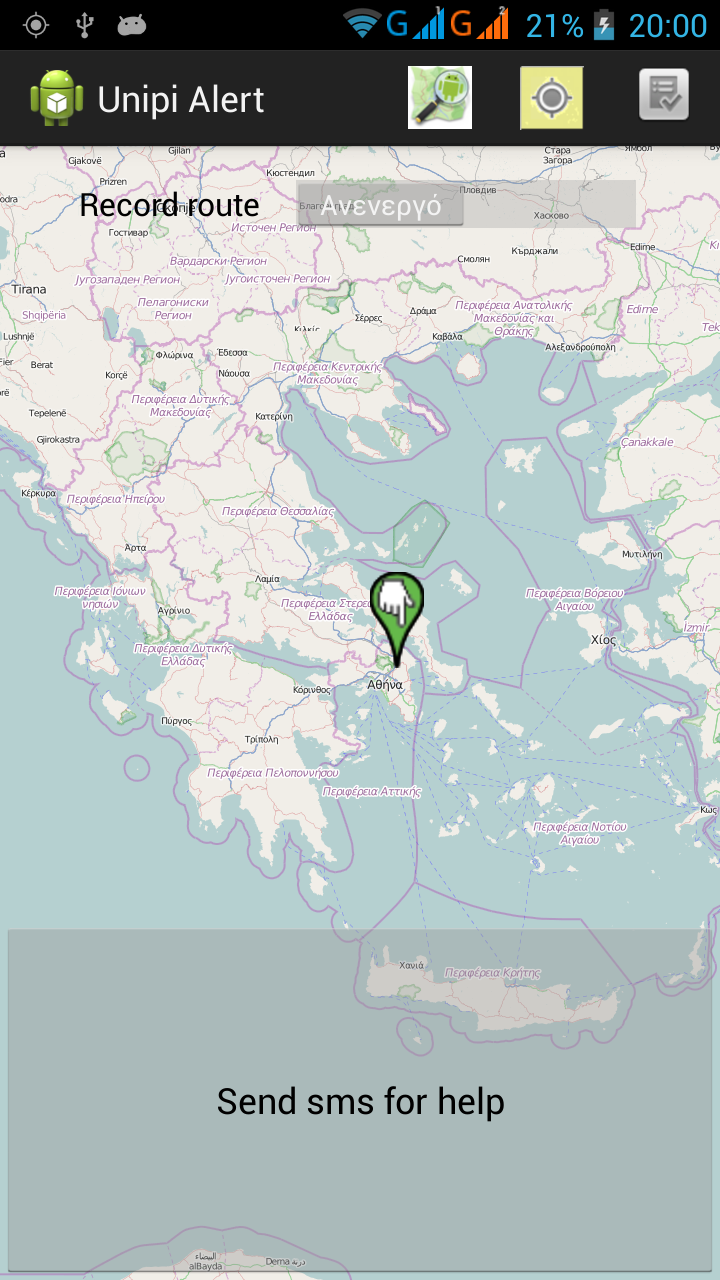
\includegraphics{images/initial_screen.png}}
\caption{Η κεντρική οθόνη της εφαρμογής}
\label{fig:initial_screen}
\end{center}
\end{figure}

\begin{table}
\begin{center}
  \begin{tabular}{|m{0.20\textwidth}|m{0.70\textwidth}|}
    \hline
     
     \vspace{0.3cm}
     \resizebox*{0.20\textwidth}{!}{
     
\includegraphics{images/bth_current_position.png}}

     & Πατώντας το συγκεκριμένο εικονίδιο μεταβαίνουμε στην τρέχουσα θέση του χρήστη. \\ \hline

     \vspace{0.3cm}
     \resizebox*{0.20\textwidth}{!}{
     
\includegraphics{images/btn_route.png}}

     & Πατώντας το συγκεκριμένο εικονίδιο ανοίγει το μενού στο οποίο φαίνονται οι καταγραφείσες διαδρομές. \\ \hline

     \vspace{0.3cm}
     \resizebox*{0.20\textwidth}{!}{
     
\includegraphics{images/btn_tracking_off.png}}

     & Πατώντας το συγκεκριμένο εικονίδιο κάθε φορά που ο χρήστης αλλάζει τοποθεσία, η οθόνη αλλάζει αυτόματα "ακολουθώντας" τον χρήστη (\en{tracking mode}). \\ \hline

     \vspace{0.3cm}
     \resizebox*{0.20\textwidth}{!}{
     
\includegraphics{images/btn_tracking_on.png}}

     & Η απενεργοποίηση του \en{tracking mode}. \\ \hline
    \hline
  \end{tabular}
\caption{Τα εικονίδια της εφαρμογής}
\label{table:icons}
\end{center}
\end{table}

\section{Επιλογές}

Για την καταχώρηση του τηλεφωνικού αριθμού στον οποίο θα στέλνετε το μήνυμα της εκτάκτου ανάγκης ο χρήστης πρέπει να πάει στο μενού των επιλογών (βλ. σχήμα \ref{fig:settings}). Εκεί καταχωρεί το τηλέφωνο στο οποίο θα στέλνονται τα μηνύματα. Δεν προτιμήθηκε να χρησιμοποιηθεί κάποια βάση δεδομένων για να στέλνονται μηνύματα σε πολλούς χρήστες διότι απλώς δεν μπορεί να απεικονιστεί εύκολα από το μενού των επιλογών. Γι` αυτό τον λόγο (αλλά και για την εκμάθηση της δημιουργίας μενού επιλογών) προτιμήθηκε να στέλνεται μήνυμα μόνο σε ένα νούμερο.

\begin{figure}
\begin{center}
\resizebox*{!}{0.9\textwidth}{
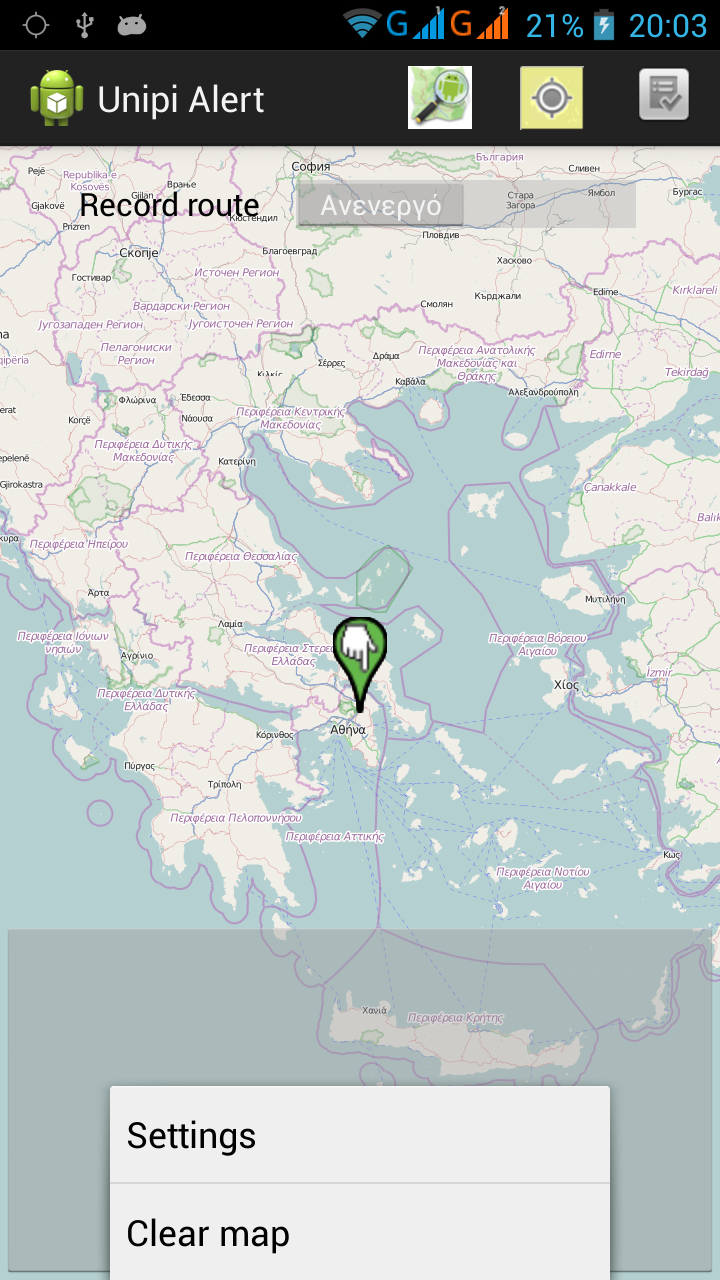
\includegraphics{images/settings.png}
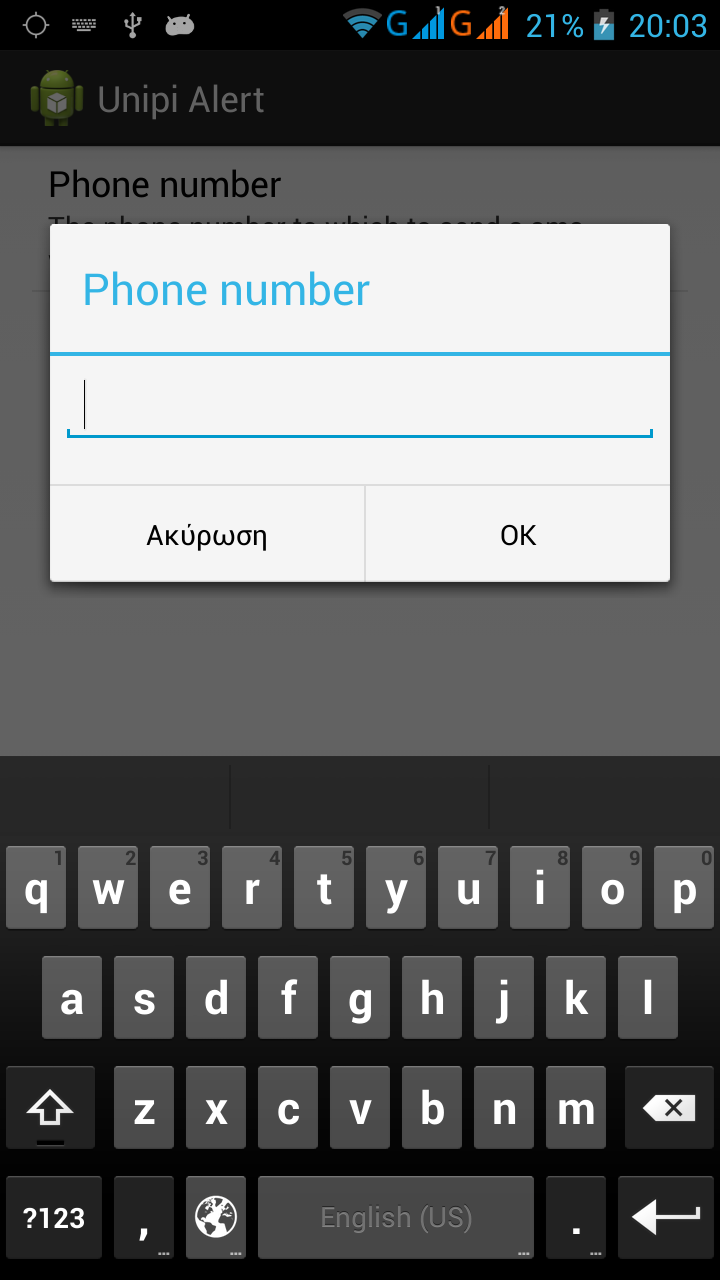
\includegraphics{images/settings_phone_number.png}
}
\caption{Η οθόνη επιλογών}
\label{fig:settings}
\end{center}
\end{figure}

Ακόμα αν δεν έχει οριστεί αυτό το πεδίο, τότε κάθε φορά που ο χρήστης πατάει το κουμπί της αποστολής του εμφανίζεται μήνυμα σφάλματος (βλ. σχήμα \ref{fig:settings_fail}). 

\begin{figure}
\begin{center}
\resizebox*{!}{0.9\textwidth}{
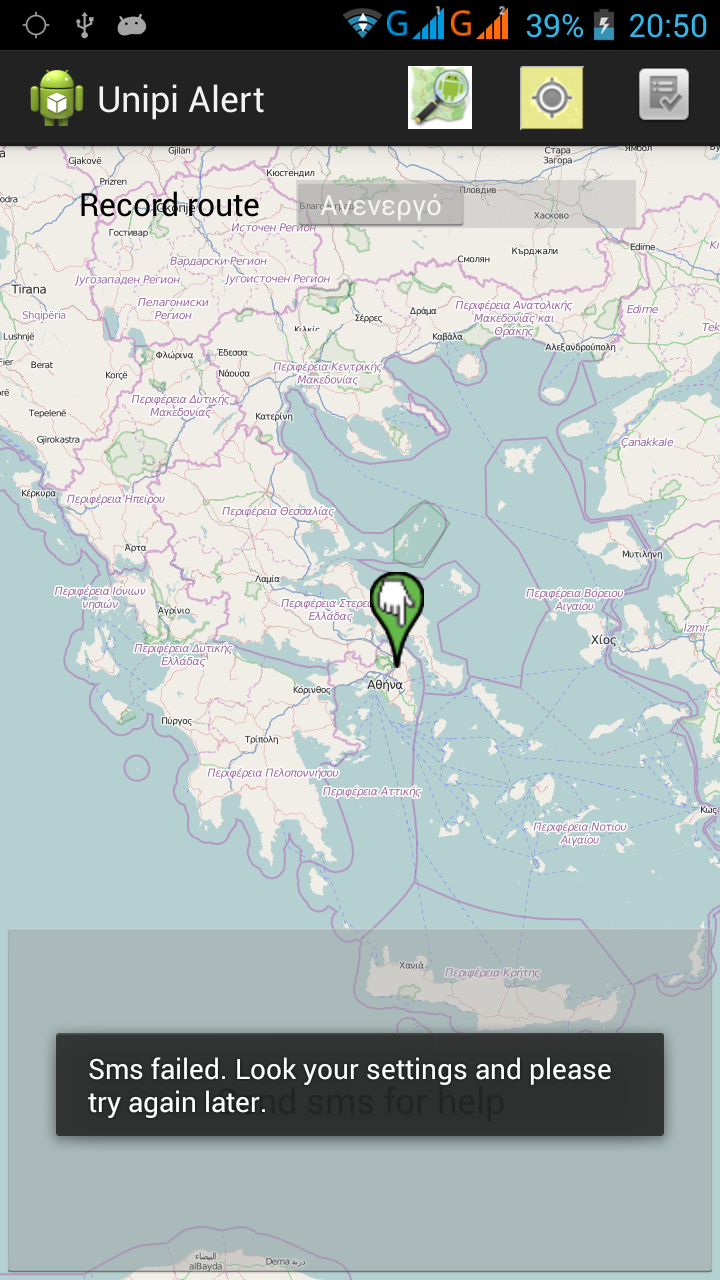
\includegraphics{images/settings_fail.png}
}
\caption{Μήνυμα σφάλματος}
\label{fig:settings_fail}
\end{center}
\end{figure}

\section{Διαδρομές}

Στην αρχική οθόνη υπάρχει συρόμενο κουμπί που επιτρέπει την καταγραφή της διαδρομής που ακολουθεί ο χρήστης. Οι διαδρομές που έχουν καταγραφεί φαίνονται πατώντας το πάνω δεξιό κουμπί (βλ. σχήμα \ref{fig:routes}). Επιλέγοντας κάποια διαδρομή ο χρήστης, η διαδρομή θα απεικονιστεί πάνω στον χάρτη, ενώ ακόμα μπορεί να αλλάξει το όνομα της ή να την διαγράψει πατώντας πάνω στην συγκεκριμένη διαδρομή για μερικά δευτερόλεπτα (βλ. σχήμα \ref{fig:routes_menu}). Για την υλοποίηση των διαδρομών χρησιμοποιήθηκε η βάση δεδομένων SQLite.

\begin{figure}
\begin{center}
\resizebox*{!}{0.9\textwidth}{
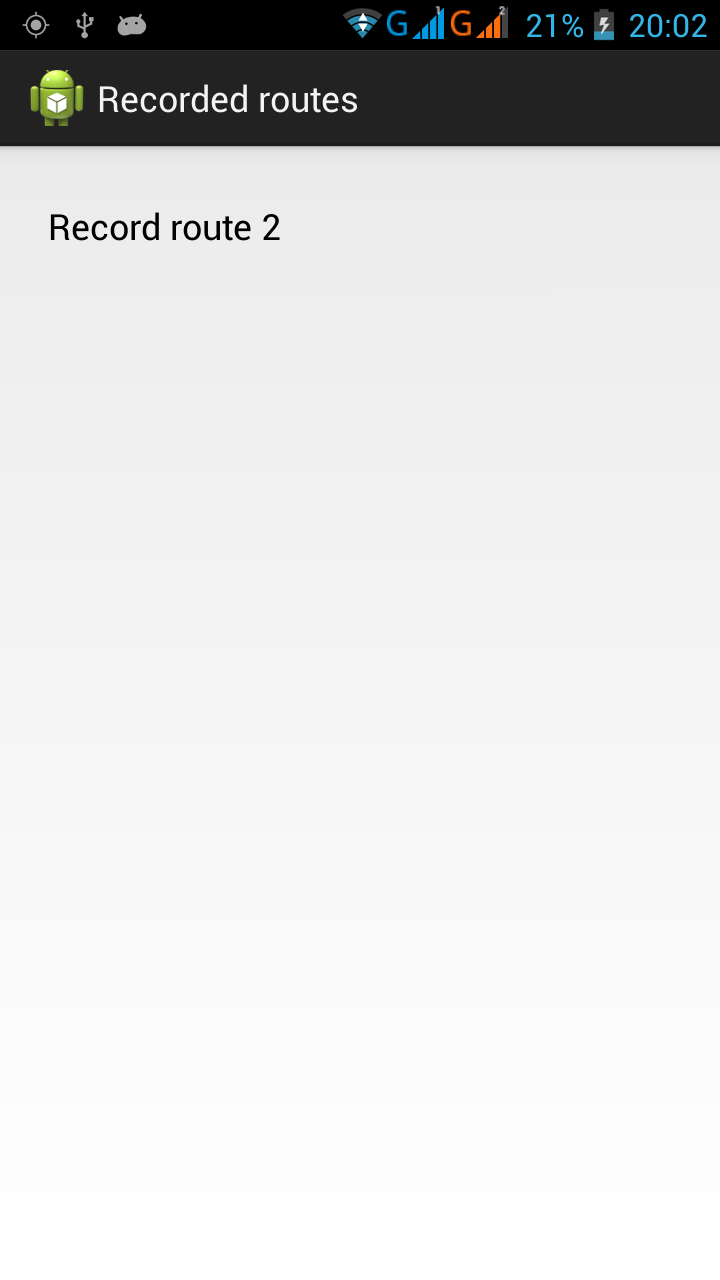
\includegraphics{images/routes.png}
}
\caption{Η οθόνη των διαδρομών}
\label{fig:routes}
\end{center}
\end{figure}

\begin{figure}
\begin{center}
\resizebox*{!}{0.9\textwidth}{
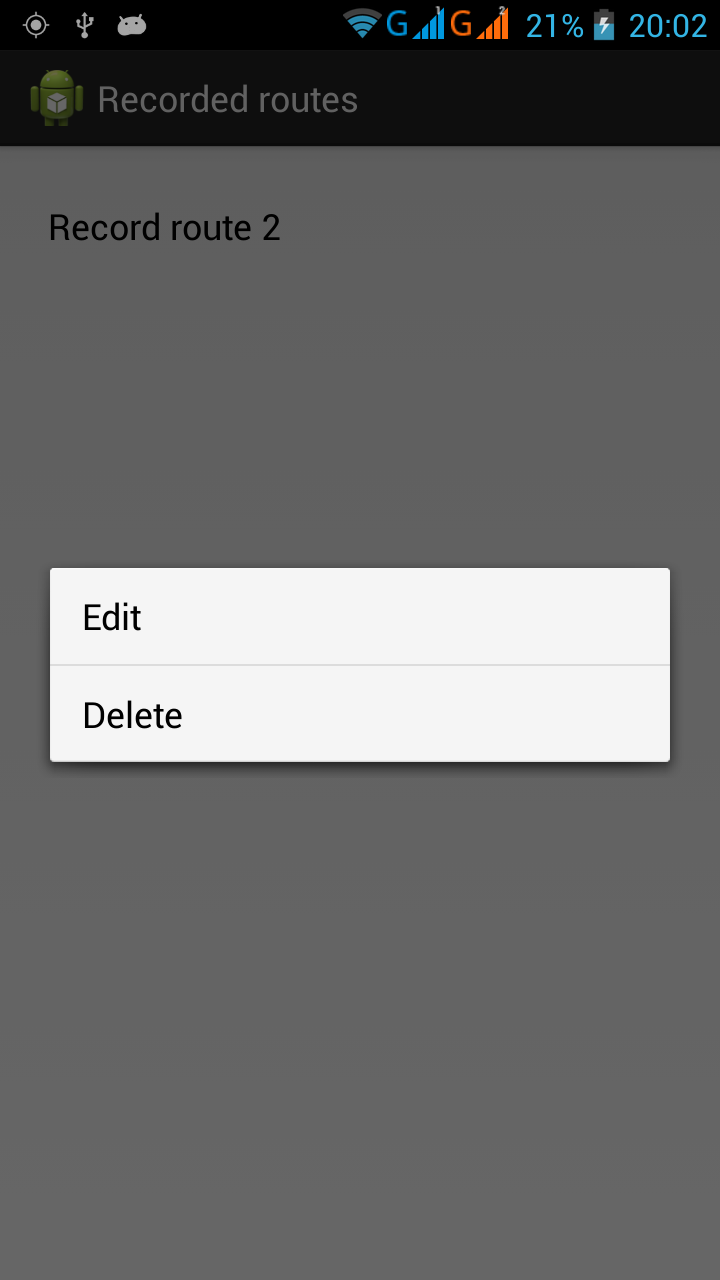
\includegraphics{images/routes_menu.png}
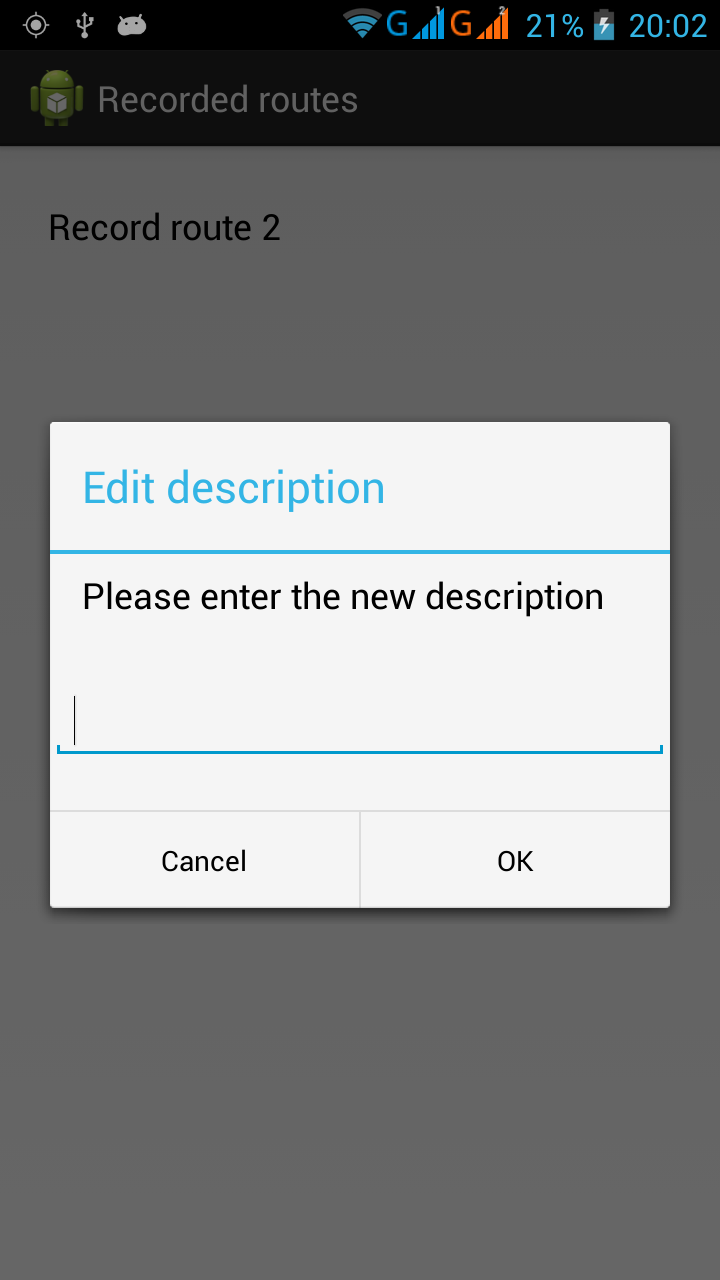
\includegraphics{images/routes_edit.png}
}
\caption{Η οθόνες επεξεργασίας των διαδρομών}
\label{fig:routes_menu}
\end{center}
\end{figure}

\newpage

\end{document}

